\vspace{-5pt}

\section{One-Round Erasure coding Atomic Storage}
\vspace{-5pt}
\begin{algorithm}[!ht]
				\begin{algorithmic}[2]
					{\footnotesize
					\begin{multicols}{2}
				
				\Statex /* at reader $r$ */
				\Operation{read}{} 
				%\State $wCounter\gets wCounter+1$
				\State $\tup{t_r, v} \gets \dagetdata{c}$
				\State $\daputdata{c}{ \tup{t_r,v}}$
				\State return $v$
				\EndOperation
				\Statex
				\Statex /* at writer $w$ */
				\Operation{write}{$v$} 
				%\State $wCounter\gets wCounter+1$
			%	\State $t_{max} \gets \dagettag{c}$
				\State $t_w \gets (t, w)$ where $t$ is machine time at $w$
		    % \State $t_w \gets (t_{max}.z+1, w)$
				\State $\daputdata{c}{\tup{t_w,v}}$
				\EndOperation
					\end{multicols}
				}
				\end{algorithmic}	
				\caption{The reader/writer steps for implementing \oreas.}\label{fig:oreas:write}
				\vspace{-1.5em}
	\end{algorithm}

Instead of logical timestamp (tags), \oreas{} relies on physical timestamps, i.e., machine time at the coordinator. The advantage of using logical timestamp is that strong consistency is guaranteed even in the presence of clock drift and absence of synchronized clocks. The downside is that it requires, as in \treasmod{}, an additional communication round in order to gather the largest tag. On the other hand, in \oreas{}, the strong consistency guarantee is reliant on correctly synchronized clocks; however, write operations complete in one round.		

\remove{Distributed systems such as Cassandra, uses machine time as the tag (physical timestamp) instead of logical tags. It is worth nothing that machine time dependent systems are susceptible to clock drift leading to violation of safety. In order to implement \treasmod{} in such systems we modify \treasmod{} to \oreas{} by modifying the client step \treasmod{} as \ref{fig:oreas:write}. \lewis{This is incorrect. we also implement ABD and TREAS into Cassandra, so it's not like we \textbf{have} to use machine time to implement the algorithm in Cassandra.}
\sout{uses tags, where  a tag $\tg{}$ is defined as a pair $(z, w)$ such that $w$ is an unique ID of the writer, and $z$ is the local machine time (when the writer issues a specific write operation). }
%Note that in Cassandra, the writer corresponds to the user proxy (i.e., a coordinator); hence, the local machine time is synchronized.
Every pair of tags can be compared in the lexicographical order. It is reasonable to use machine time in our context, since the ``client'' is a proxy server (or a coordinator), which has a synchronized clock with other servers. In fact, Cassandra uses machine time to identify new values as well. For the case that time synchronization is difficult, \treasmod{} should be implemented.  \lewis{Do we need to mention AREAS? Doesn't seem to add anything. We also implement TREAS.} \blue{This little section is tricky and we don't need to talk about ARES. Please feel free to edit or change}.}
%\blue{removed the rest of the section by using the remove command}

\remove{
%A particular form of the  strong consistency we are interested, i.e., atomicity, is composability. 
In this section, we describe our EC-based storage protocol -- One-Round Erasure coding Atomic Storage (\oreas).
One desirable property of atomicity \cite{lamport} (or linearizability \cite{herlihy1990linearizability}) is composability \cite{herlihy1990linearizability}.
That is, a collection of atomic storage units used together in an arbitrary way still satisfy atomicity. Note that some other forms of strong consistency might not have such a property. This is also why we are interested in providing atomicity. Due to composability, we describe \oreasSpace in terms of a single key-value pair (KV-pair), i.e., the key field is omitted in our discussion.
Our implementation supports multiple clients accessing multiple KV-pairs.
In our evaluation, we test CassandrEAS with multiple keys.
%We assume the value of our KV-pair is encoded, using a $MDS[n, k]$, into $n$ coded elements $c_1, c_2, \cdots c_n$ where each $c_i$ is stored at server $s_i$.  
%We provide two protocols: \treas{} and \oreas{}, whose pros and cons are described in later paragraphs.  
Due to space constraint, we briefly describe our protocol at a high-level along with the pseudo-code. %Figure \ref{fig:2} provides an illustration. 
Most technical details (including proofs) are presented in the accompanied technical report.\footnote{Our report is not currently available on web due to anonymous clause. If the paper is accepted, we will upload it to arxiv.}
The pseudo-code for readers and writers is presented in Algorithm \ref{alg:oreas-client}, and pseudo-code for servers is in Algorithm \ref{alg:oreas-server}.




%\vspace*{3pt}
%\noindent\textbf{TREAS}~~
%\subsection{OREAS}

\paragraph*{Meta-data} \oreas{} uses tags, where  a tag $\tg{}$ is defined as a pair $(z, w)$ such that $w$ is an unique ID of the writer, and $z$ is the local machine time (when the writer issues a specific write operation). 
%Note that in Cassandra, the writer corresponds to the user proxy (i.e., a coordinator); hence, the local machine time is synchronized.
Every pair of tags can be compared in the lexicographical order. It is reasonable to use machine time in our context, since the ``client'' is a proxy server (or a coordinator), which has a synchronized clock with other servers. In fact, Cassandra uses machine time to identify new values as well. For the case that time synchronization is difficult, we have another protocol, called \treas{}, which uses a logical timestamp to replace the machine time. 
For brevity, we focus on \oreasSpace in this paper.
%The detail are presented in our technical report.

\paragraph*{Write Operation} Suppose $v$ is the value that the writer intends to update the KV-pair with. The writer (or writer proxy) encodes $v$ to coded elements $c_1, c_2, \cdots c_n$, along with tag $\tg{}$, and sends the corresponding element to each server. Every server that receives a coded element
stores the coded element in its $List$ and performs garbage collection (i.e., replacing elements with smaller tags or storing a pair with $\perp$ value field). Finally,
% garbages collect the store coded element in its $List$ if the  corresponding tag is smaller than $t_{max}$ and 
it sends an acknowledgment message back to the writer. Once the writer receives acknowledgments from $\lceil\frac{n+k}{2}\rceil$  servers, it completes the write operation.

\paragraph*{Read Operation} The reader (or reader proxy) requests all servers for the lists of values. Upon receiving the request,  a server sends its local variable $List$ containing $(t, c_i)$ or $(t, \bot)$ to the reader.  
%\red{There are at most $\delta$ of them in the list???}. \blue{Each server stores in $List$  all the tags that it receives in the execution; even if the coded element corresponding to a tag $t$ is garbage collected, the server stores a tuple of the form $(t, \bot)$ } 
Once the reader receives responses from  $\lceil\frac{n+k}{2}\rceil$ of the servers, it decodes the value $v$ corresponding to the tag $t_{max}$. 
Our protocol ensures that as long as the number of crashed servers is  $\leq f$ and the number of concurrent writes is $\leq \delta$, a value is always decodable, and atomicity is satisfied.
Next the reader computes the coded elements of $v$, and together with the servers executes the steps as in the write operation (i.e., write-back phase), and then completes the read operation.  %Note that we have argued analytically that as long as the system does not experience concurrency more than $\delta$, the reads will always decode correctly. 


\paragraph*{Correctness}
We prove our protocols satisfy strong consistency (atomicity) in our technical report. We also develop a consistency checker based on the approach specified in \cite{Lynch1996} to ensure that our implementation also provides this guarantee. Validating strong consistency requires precise clock synchronization across all servers, since it needs to use global clock to ordering operations and events. This is impossible to achieve in a distributed system where clock drift is inevitable. To circumvent this, we deploy our CassandrEAS servers on a single machine and use Mininet \cite{MininetWebsite} to simulate the underlying network communication. Our checker then uses the machine time as the global clock. We collect multiple traces of 20,000 operations under different configurations with potentially machine failures. The checker verifies that all traces we tested satisfy strong consistency.
%so that every process observers the same clock running in the VM. 

%Our checker gathers meta-data regarding an execution of operations, such as start and end times, and timestamps.
%, and this data includes start and end times of all the operations, as well as other parameters like logical timestamps used by the protocol. 
%The checker logic is based on the conditions appearing in Lemma 13.16~\cite{Lynch1996}, which provide a set of sufficient conditions for guaranteeing strong consistency. The checker validates strong consistency property for ever KV-pair individually for the execution under consideration. We collect multiple traces of 20,000 operations under different configurations with potentially machine failures. The checker verifies that all traces we tested satisfy strong consistency.


%\paragraph{OREAS} %The implementation of OREAS is as follows, where instead of the logical tags we rely on physical timestamps, i.e., machine time at the coordinator.

%\emph{read} The read operation of OREAS is similar to that of TREAS. 

%\emph{write} The primary difference between TREAS and OREAS is that TREAS uses logical time stamp (or tag) where as OREAS uses the physical time at the write client  as the largest tag.  As a result, in OREAS th write operation simply involves using the current physical time to tag the  coded elements to a set of $  $ servers. Therefore, it does not need any round to recover the largest tag at the server 
%\vspace*{3pt}
%\noindent\textbf{OREAS}~~
%\subsection{OREAS}
%Instead of logical timestamp (tags), \oreas{} relies on physical timestamps, i.e., machine time at the coordinator. The advantage of using logical timestamp is that strong consistency is guaranteed even in the presence of clock drift and absence of synchronized clocks among the various servers.  The downside is that it requires, as in \treas{}, an additional communication round in order to gather the largest tag, which increases latency. On the other hand, in  \oreas{}, the strong consistency guarantee is reliant on correctly synchronized clocks; however, write operations complete in one round.
%In our setting every server stores only one, corresponding to the most recent tag received, coded element of dimension $\lceil\frac{k}{\delta+1}\rceil$. Therefore, there is no explicit garbage collection required.

%\paragraph{Storage cost}
%\vspace*{3pt}
%\noindent\textbf{Storage cost}~~
\paragraph*{Storage Cost}
In \oreas{}, erasure coding is used, and each server stores a list of all the tags that it has received so far. If a server receives the coded element corresponding to a tag newer than the current KV-pair with timestamp $t$, the server would update the current KV-pairs to the form $(t, \bot)$. The key feature that is different from other EC-based algorithms (e.g., \cite{dimakis2010network, rashmi2016ec, tamo2014family,GIZA2017,CadambeLMM17, SODA2016, LDS2017,Cocytus2016}) is that each server stores \emph{exactly one coded element} in $List$ and the rest of the elements in $List$ are of 
the form $(t', \bot)$, where $t'$ is some tag or timestamps that were garbage collected and $\bot$ is a place holder for null data. The  cost of storing one value of unit size at each server is hence $\frac{1}{ \lceil\frac{k}{\delta+1}\rceil}$. Recall that $\delta$ is
the maximum number of writes concurrent with any read operation, and $k = n-2f$.

\myparagraph{Storage and Communication Costs for \treasmod{}.}
\nn{We now briefly present the storage and communication costs associated with {\treasmod{}}. %Due to space limitations the proofs appear in \cite{}.
	Recall that by our assumption, the storage cost counts the size (in bits) of the coded elements 
	%that are locally stored, which are 
	stored in the $List$ variable at each server. We ignore the storage cost due to meta-data and temporary variables.
	Also, for the communication cost we measure the bits sent on the wire between the nodes.
}
\nn{
	\begin{theorem}\label{treas:performance}
		The \treasmod{} algorithm has: (i) storage cost $(\delta +1 )\frac{n}{k}$, (ii) communication 
		cost for each write at most to $\frac{n}{k}$, and (iii) communication 
		cost for each read at most $(\delta +2)\frac{n}{k}$.
	\end{theorem}
}
}
%\begin{theorem} \label{thm:storage_TREAS}
%	The worst-case total storage cost of \treasmod{} algorithm is  $(\delta +1 )\frac{n}{k}$.
%\end{theorem}
%\proofremove{
%	\begin{proof}
%		The maximum number of  (tag, coded-element) pair in the $List$ is $\delta+1$, and the size of each coded element is 
%		$\frac{1}{k}$ while the tag variable is a metadata and therefore, not counted. So, the total storage cost is $(\delta +1)\frac{n}{k}$.
%	\end{proof}
%}
%
%We next state  the communication cost for the write and read operations in  \treasmod{}. Once again, note that we ignore the communication cost arising from exchange of meta-data.
%
%\begin{theorem} \label{treas:write_cost}
%	The communication cost associated with a successful  write operation in \treasmod{} is at most $\frac{n}{k}$. 
%\end{theorem}
%\proofremove{
%	\begin{proof}
%		During read operation, in the $\act{get-tag}$ phase the servers responds with their highest tags variables, which are metadata. However, in the $\act{put-data}$ phase, the reader sends each server the  coded elements of size  $\frac{1}{k}$ each, and hence the total cost of communication for this is $\frac{n}{k}$. Therefore, we have the worst case communication cost of a write operation is $ \frac{n}{k}$.
%	\end{proof}
%}
%\begin{theorem} \label{radonc:read_cost}
%	The communication cost associated with a successful read operation in \treasmod{} is at most $(\delta +2)\frac{n}{k}$. 
%\end{theorem}
%\proofremove{
%	\begin{proof}
%		During read operation, in the $\act{get-data}$ phase the servers responds with their $List$ variables and hence each such list 
%		is of size at most $(\delta +1)\frac{1}{k}$, and then counting all such responses give us $(\delta +1)\frac{n}{k}$.  In the $\act{put-data}$ phase, the reader sends each server the  coded elements of size  $\frac{1}{k}$ each, and hence the total cost of communication for this is $\frac{n}{k}$. Therefore, we have the worst case communication cost of a read operation is 
%		$(\delta+2) \frac{n}{k}$.
%	\end{proof}
%}
%

\section{Our System: CassandrEAS}
\label{s:CassandrEAS}

\subsection{Implementation}
We share our implementation experience here in hope to lower the barrier of implementing other replication- or EC-based protocols in Cassandra in the future.\footnote{We also has a separate paper that documents the implementation and benchmarking of other replication-based storage protocols in Cassandra \cite{Tseng_Cass}.}
We have two main goals in our implementation: (i)
make minimum modification to the original Cassandra codebase; %, e.g., using Cassandra's original way of communication between servers; 
%For example, we try not to introduce new complicate data structure; and 
 (ii)
allow Cassandra users to use our implementation \textit{without} knowing the details of \oreas. That is, users can use the same Cassandra API in our system. 
The implementation turns out to be a difficult task because we are constrained to using only Cassandra's internal tools and data structures for communication and coordination. We spent enormous amount of time to decompose and understand Cassandra's internal logic because the codebase is not well documented and often provide poor comments. 
The version of Cassandra (version 3.11) that we used to develop contains around 57,000 LoC in Java. 
We also implemented the algorithm \treas, which uses logical timestamp to deal with loosely synchronized clock.
Our implementation of both algorithms consists of around 2,000 LoC. We did not implement our protocols as a middleware because the protocols require system information (e.g., timestamps), which is not revealed externally.

\noindent\textbf{Data Model}~~Cassandra adopts the column-family data model, which provides a richer functionalities than a simple read-write object (KV-pair).  At a high level, Cassandra's data structure can be viewed as a table, where each row corresponds to data sharing the same key.
CassandrEAS uses a row to store one KV-pair.
Recall that the maximum number of writes concurrent with any read is denoted by $\delta$. 
We use $2+2\delta$ columns for each row: key, value (a place holder for original data), and additional $2\delta$ columns for each version of the write.
For each version, we use one column for timestamp (either physical or logical timestamp), and the other for the corresponding coded element.
The reason that we need the value column is that it allows Cassandra to return the original data (decoded element) to the client. That column does \textit{not} store any data in storage. Each server only stores one coded element. The rest would be $\perp$ as discussed previously.



%\vspace{3pt}
%\noindent\textbf{Data Model}~~
%%%%%%%%%%%%%%%%%%%%%%%%%%%%%%%%%% DO I NEED THIS??? %%%%%%%%%%%%%%%%%%%%%%%%%%%%%%%%%%
%\paragraph*{Data Model}
%Cassandra adopts the column-family data model, which provides a richer functionalities than a simple read-write object (KV-pair).  At a high level, Cassandra's data structure can be viewed as a table, where each row corresponds to data sharing the same key. CassandrEAS uses a row to store one KV-pair. Recall that the maximum number of writes concurrent with any read is denoted by $\delta$.  We use $2+2\delta$ columns for each row: key, value (a place holder for original data), and additional $2\delta$ columns for each version of the write. For each version, we use one column for timestamp (either physical or logical timestamp), and the other for the corresponding coded element. The reason that we need the value column is that it allows Cassandra to return the original data (decoded element) to the client. That column does \textit{not} store any data in storage. Each server only stores one coded element. The rest would be $\perp$ as discussed previously.

%Also since Erasure Encoding needs to ensure order, we assign an individual id number to the individual node. In our Schema, node\_ID starts at 1 and ends at the number of servers.


%In Cassandra, user first contacts the coordinator (or client proxy), and the coordinator follows the replication algorithm to read or write the data on the behalf of the Cassandra user. In other words, coordinator \textit{is} the client with respect to the replication algorithm. Therefore, in the presentation below, we will use coordinator and client interchangeably. In Cassandra's design (more specifically, the consistent hashing protocol), each server is a coordinator handling a certain set of keys.
%\vspace{3pt}
%\noindent\textbf{Technical Details}~~
\paragraph*{Technical Details}
We mainly modify the following two files in the Cassandra codebase. 
In Cassandra's terminology, ``mutation'' is essentially a write operation that modifies the internal state of the servers.
(i) \textit{StorageProxy.java} is where the coordinator server handles the user's read or write operation. Specifically,
\textsc{mutate} function handles Cassandra user's write operation whereas \textsc{fetchRows} function handles user's read operation. 
The size of read/write quorums is also specified in this file; and (ii) \textit{MutationVerbHandler.java} where each server's database engine handles incoming write requests from the coordinator.
Specifically, \textsc{doVerb} function applies the mutation onto local storage. One major challenge we encountered is that Cassandra does \textit{not} provide an easy way to fetch users' requests and modify their mutations.
We have to figure out a way to construct a new mutation when we need to add new fields such as timestamp and coded elements.
Recall that we do not want to introduce new data structure, so we choose to use Cassandra's column family data model (i.e., an ordered collection of rows) to store the List variable at each server.
%\vspace{3pt}
%\noindent\textbf{Erasure Coding}~~
%\subsection{Erasure Coding}
CassandrEAS uses BackBlaze Reed-Solomon Code.%\footnote{https://github.com/Backblaze/JavaReedSolomon}  These details are presented in our technical report.


\begin{figure*}[!ht]
	\begin{subfigure}[b]{0.32\textwidth}
		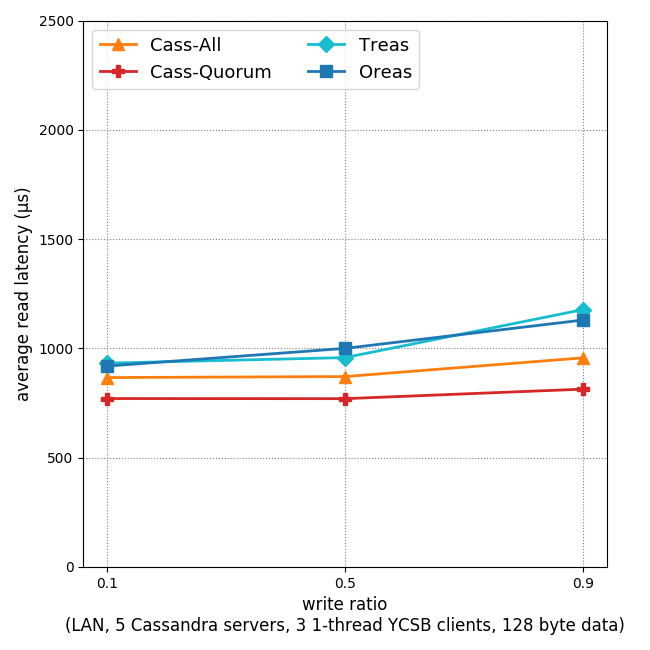
\includegraphics[width=0.9\linewidth]{img/LAN_7_latency,_vary_write,_5_svrs,_average_read.png}
		\caption{average read latency vs. write ratio}
		\label{fig:latency-read-ratio-avg}
	\end{subfigure}
	\hfill %%
	\begin{subfigure}[b]{0.32\textwidth}
		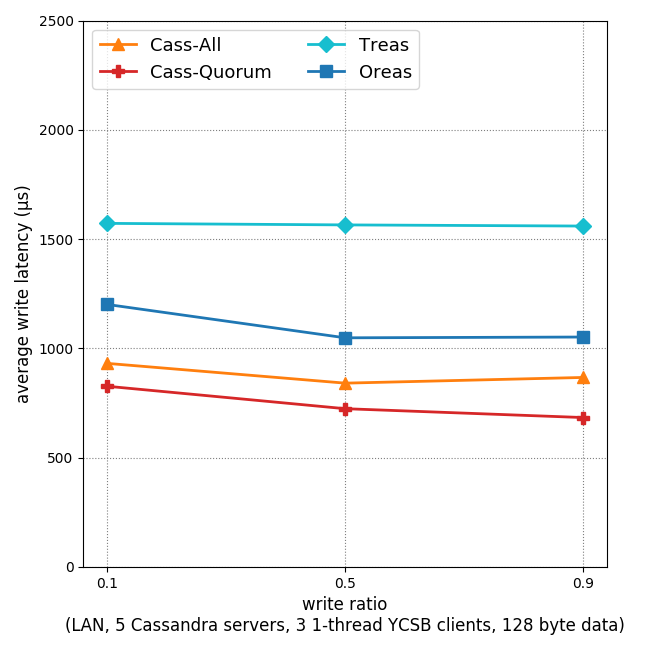
\includegraphics[width=0.9\linewidth]{img/LAN_9_latency,_vary_write,_5_svrs,_average_write.png}
		\caption{average write latency vs. write ratio}
		\label{fig:latency-write-ratio-avg}
	\end{subfigure}  
	\hfill %%
	\begin{subfigure}[b]{0.32\textwidth}
		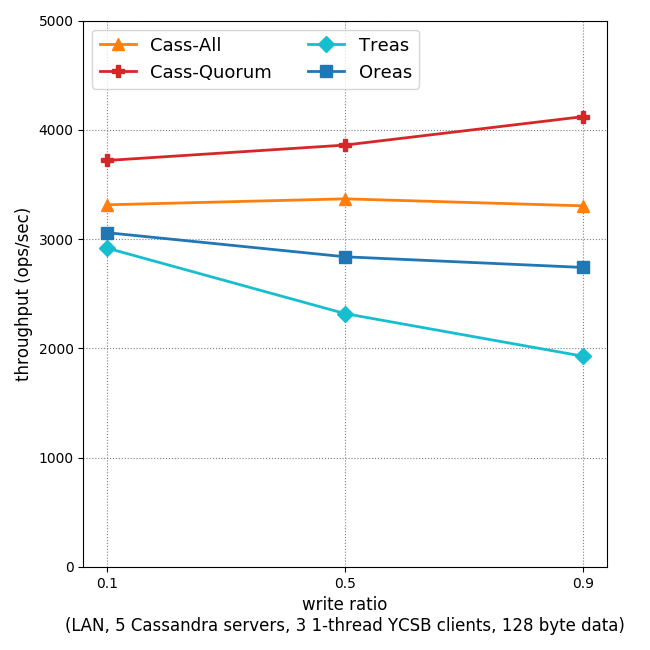
\includegraphics[width=0.9\linewidth]{img/LAN_6_throughput,_vary_write,_5_svrs.png}
		\caption{throughput vs. write ratio}
		\label{fig:throughput-ratio}
	\end{subfigure}

	\begin{subfigure}[b]{0.32\textwidth}
		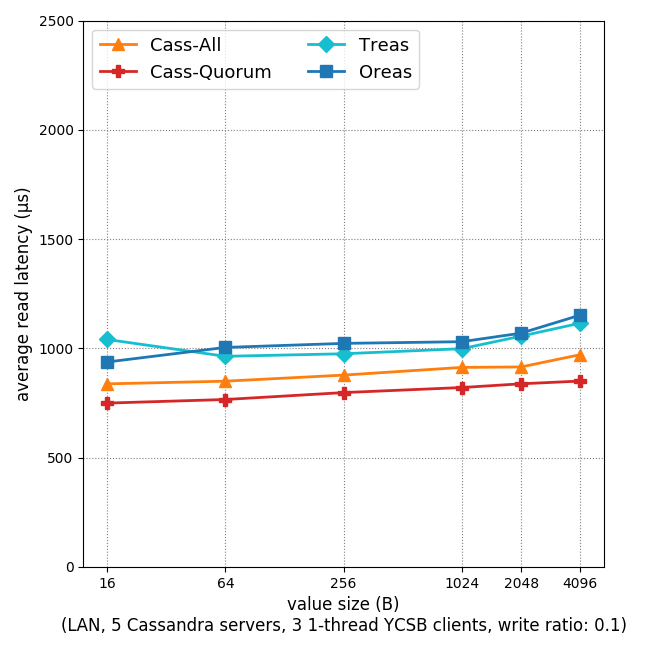
\includegraphics[width=0.9\linewidth]{img/LAN_12_latency,_vary_size,_5_svrs,_average_read.png}
		\caption{avg read latency vs. data size}
		\label{fig:latency-read-size-avg}
	\end{subfigure}    	
	\hfill
	\begin{subfigure}[b]{0.32\textwidth}
		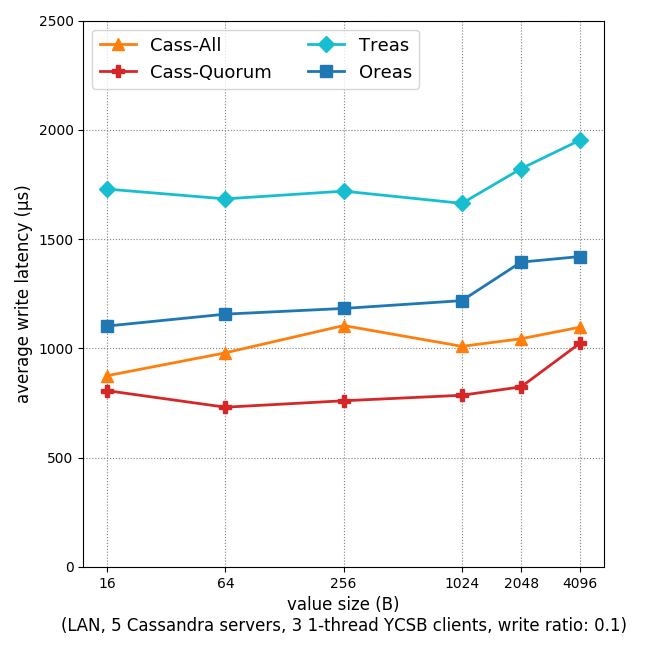
\includegraphics[width=0.9\linewidth]{img/LAN_14_latency,_vary_size,_5_svrs,_average_write.png}
		\caption{avg write latency vs. data size}
		\label{fig:latency-write-size-avg}
	\end{subfigure}    	
	\hfill %%	
	\begin{subfigure}[b]{0.32\textwidth}
		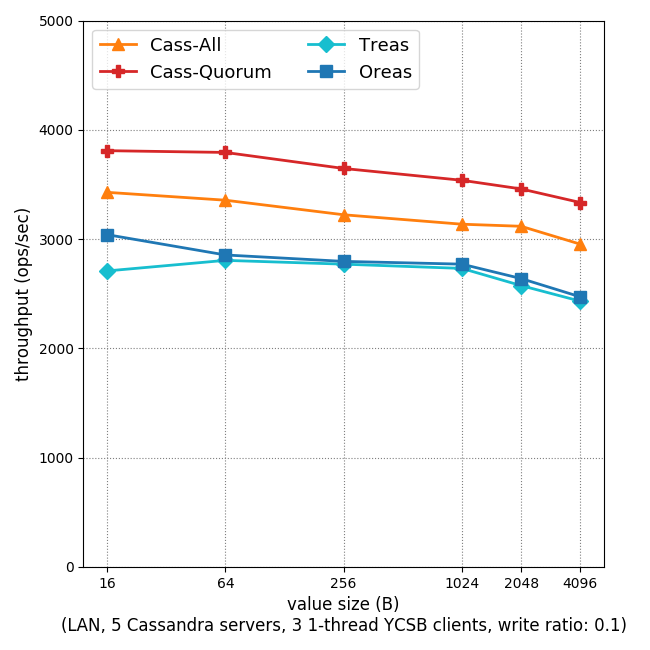
\includegraphics[width=0.9\linewidth]{img/LAN_11_throughput,_vary_size,_5_svrs.png}
		\caption{throughput vs. data size}
		\label{fig:throughput-size}
	\end{subfigure}    
	%	\hfill DON"T SHOW THIS ==> need to argue about inconsistent result for the %%%
	%	\begin{subfigure}[b]{0.3\textwidth}
	%		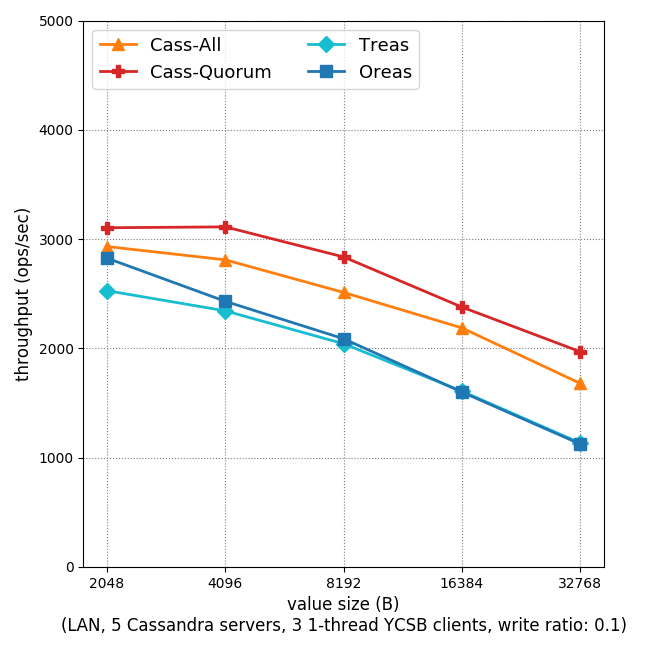
\includegraphics[width=0.9\linewidth]{img/LAN_16_throughput,_vary_size,_5_svrs.png}
	%		\caption{throughput vs. large data size}
	%		\label{fig:throughput-size-large}
	%	\end{subfigure}    	
	\caption{Comparison of latency and throughput of different configurations}\label{fig:evaluation} 
	\vspace{-10pt}
\end{figure*}
%\section{CassandrEAS: Evaluation}
\vspace{-5pt}

\subsection{Evaluation}
\label{s:evaluation}
\vspace{-3pt}

We evaluate the performance of CassandrEAS by comparing it to vanilla Cassandra (version 3.11). 
Cassandra-All requires the coordinator to hear from every server, whereas Cassandra-Quorum only requires to hear from a majority.

%and Cass-ABD. Cass-ABD replaced Cassandra's replication protocol with ABD \cite{ABD96}, which is a storage algorithm based on logical timestamps.
%We present the highlights of our evaluation results below:

%\begin{itemize}
%	\item \red{What should be here?}
%\end{itemize}

%\subsection{Experimental Setup}

%\paragraph{Cluster Configuration}
%\vspace*{3pt}
%\noindent\textbf{Cluster Configuration}~~
\paragraph*{Cluster Configuration and Workload}
We use the Google Cloud Platform (GCP) as our testing platform.
Each virtual machine (VM) is equipped with 4 virtual CPUs, 16 GB memory, and hosting Ubuntu 14.04 LTS.
All VMs are located in datacenter us-east1-c (South Carolina).
VMs use internal IP’s for communication.
The average RTT between any two VMs is around $0.3$ ms, and TCP bandwidth measured by Iperf is around $7.5$ Gbits/sec. %We use ping to estimate RTT.
For most of evaluation, our cluster consists of 5 VMs, and 3 YCSB single-threaded clients. Thus, $\delta = 3$.
We use YCSB to generate realistic workload. We first insert a total of 30,000 KV-pairs, and each user performs 100,000 read or write operations. Recall that we have 3 YCSB clients, so we have 300,000 operations in total. We report the aggregated throughput, i.e., the sum of total operations per second across three YCSB clients. %We use the ``default Workload A'' provided by YCSB, whose operations follow Zipfian distribution.

%We use the Yahoo! Cloud Serving Benchmark (YCSB) \cite{YCSB} for evaluation. We did not choose Cassandra's own stress test tool, because it does not provide a straightforward way to disable Batch operation. Furthermore, it uses auto-generated data for all columns predefined.
%All of our YCSB workloads are modified from the ``default Workload A'' -- read-update workload. That is, YCSB first issues all-key insert before benchmarking, and we only benchmark on the read/update performances. 

%\vspace{3pt}
%\noindent\textbf{Performance}~~
\paragraph*{Performance}
Figure \ref{fig:evaluation} presents our evaluation results in different configurations.
Figures \ref{fig:latency-read-ratio-avg} to \ref{fig:throughput-ratio} show latency and throughput under different write ratio with data size equal to $128 B$. Read latency is comparable across all four algorithms. \treas{} has poor write latency due to the usage of logical timestamps, which requires an extra round-trip. \oreas{} has moderate penalty in write latency. 
Throughput is comparable in the case of write ratio $0.1$, a common case in NoSQL KV-stores.
Figures \ref{fig:latency-read-size-avg} to \ref{fig:throughput-size} show latency and throughput under different data size with write ratio $0.1$. We only show average latency, as 95 percentile has the same pattern.  Figure \ref{fig:throughput-size} demonstrates that CassandrEAS suffers moderate penalty on throughput.

%If we compare Figures \ref{fig:throughput-size} and \ref{fig:throughput-ratio}, then we see small discrepancy between throughput numbers. These two sets of experiments were conducted on different days. We have observed that performance can vary by around $10\%$ in different days with GCP. However, we are fairly confident that our evaluation methodology eliminates potential biases and noises. 

%Our evaluation results demonstrate that CassandrEAS provides latency and  throughput comparable to Cassandra in some cases. The average and 95 percentile latency numbers for reads and writes are shown in Fig~\ref{fig:evaluation} . The plots for throughput of operations under various value sizes and read to write frequency ratios further substantiates that there is no blocking operations due various workload properties. We obtained similar availablity and throughput results when we introduce server crashes. 

%\paragraph{Availability and Fault-tolerance}
%\vspace{3pt}
%\noindent\textbf{Aavailability and Fault-tolerance}~~
\paragraph*{Availability, Fault-tolerance, and Scalability}
CassandrEAS is highly available, fault-tolerant, and scalable, because its core is based on Cassandra.
It can continue serving client's operations as long as the conditions specified by $f$ and $\delta$ are satisfied.
We have tested our system with 7 servers and 1 crashed server, and observed minimal disruption on throughput (ranging from $0.1\%$ to $2.5\%$ decrease). We also observed that each YCSB client's throughput decreased a bit right after a server crashed, and later came back to normal throughput (compared with a cluster without any fault). Finally, we also tested clusters with 7, 9, and 11 servers. The throughput of \oreasSpace is in the range of $77 - 80 \%$ of Cassandra's. This demonstrates that CassandrEAS' performance is also scalable, i.e., the throughput increases when $n$ increases.
%some data with n=7, delta=3, 16B, w/r = 0.1
%name     throughput
%Treas-f=0 2682.11
%Treas-f=1 2610.55
%Oreas-f=0 2702.34
%Oreas-f=1 2697.6
%Indeed, the throughput just decreased a little bit. I also observed that the throughput at each YCSB client decreases 100-200 ops/sec for less than 10 seconds then comes back as normal.


\paragraph*{Correctness}
We develop a consistency checker based on the approach specified in \cite{Lynch1996} to ensure that our implementation also provides this guarantee. Validating strong consistency requires precise clock synchronization across all servers. %, since it needs to use global clock to ordering operations and events. 
This is impossible to achieve in a distributed system where clock drift is inevitable. To circumvent it, we deploy our CassandrEAS servers on a single machine and use Mininet \cite{MininetWebsite} to simulate the underlying network communication. Our checker then uses the machine time as the global clock. We collect multiple traces under different configurations with failures. The checker verifies that all traces we tested satisfy atomicity.

\vspace{-3pt}
\section{Summary}

Strong consistency, storage efficiency, and availability are three key features for NoSQL KV-stores. We demonstrated that through  CassandrEAS -- erasure coding can be used to reduce storage cost while incurring moderate performance penalty. One interesting future work is to investigate how to apply \treasmod{} and \oreas{} in other NoSQL KV-stores, or to Cassandra to support transaction-related primitives.\vspace{-3pt}
